\chapter{Introduction} % Main chapter title

\label{introduction} % Change X to a consecutive number; for referencing this
% chapter elsewhere, use \ref{ChapterX}

\lhead{Chapter 1. \emph{Introduction}} % Change X to a consecutive number; this
% is for the header on each page - perhaps a shortened title

\section{Introduction}

Model Driven Engineering has been a part of computer sience since the very
beginning, where models has been used to raise the level of abstraction for
various problems or by describing parts of a computer system. Model Driven
Engineering has been part of computer sience Model Driven Engineering
(MDE)\cite{France2007} thrives to raise the level of abstraction in program
specification and increase automation in program development. The main idea in
MDE is to use models at different levels of abstraction when developing
applications. This leads to a higher level of abstraction in program and
problem specification. This level of abstraction is obtained either through
extensive use of models to describe some design patterns in a software
application or through use of standardized models. The first option is probably
an element of MDE that is most common among software engineers. That you
implement some aspect of a system based on a model.
Unified Modelling Language is an example of a modelling language often used to describe
system design patterns in an application domain. The second principle of Model
Driven Engineering is to increase automation in program development, and to
obtain this we use something called model transformations. 

A model transformation is when we change some source model from one
instance to another instance and end up with a target model. We can
distinguish these operations into either endogenous or exogenous model
transformations. In an endogenous model transformation we take one model
expressed in a language and produce a model expressed in the same language.
While in an exogenous model transformation we start with a model
expressed in one language and translate this into a model expressed in another
modelling language. It is essential that these models are consistent. This is
obtained through the use of metamodels. A metamodel is a description of a
model, where it defines elements that are used in the model. Models in a system
is consistent if the source and target model corresponds to a metamodel. This
way system developers can safely presume that a model has changed accordingly
to its metamodel and therefore is consistent. A target model can produce two
different kind of output models. The first one is code generation, often
referred to Model to Text(M2T) transformation, and it takes one model and
produces implementation code. This is convenient if for example a software
engineer wants to produce source code from a given model. The latter is often
referred to Model to Model(M2M) transformations. M2M transformations take a
model as input and produces a model as output. In this article we try and go
into depth for some model to model transformation tools. These tools are
The Henshin project\cite{Henshin}, Attributed Graph Grammer System (AGG)
\cite{AGG} and ATLAS Transformation Language (ATL) \cite{ATL}. Henshin and AGG
is build around the algebraic concepts of graph transformations. Whereas ATL
transformation language is a syntax based transformation language that relies
on manual coding to create model to model transformations. In this paper we
will look at a specific example of a model to model transformation, where we
are going to translate from a Activity diagram to a Petri Nets model and
evaluate how this example performs for different tools. When we have applied
this example to the different tools, we will try and find both strengths and
weaknesses for these tools. In the next section, we will shortly describe the
two models that are involved in this model to model transformation. Then in
chapter 2 we will look at what graph transformation is. Model transformations
is still a subject of research, and to use graph transformation or graph
rewriting is the most common tool used at this moment to handle model to model
transformation problems for graph based models. In chapter 3, 4 and 5 we will
look at these three different tools. Where we will shortly describe how editing
model to model transformation is handled. If its either a graphical editor or a
syntax based editor. We will also describe how these three tools handle
consistency and metamodels. And in the final chapter, we will evaluate these
tools. Where we will look at strength and weaknesses. But before we go into
depth in these tools, we have to specify the test case for this paper.

\subsection{Problem specification}
\noindent The task was to take a certain instance of a model to model
transformation, in this case translating an activity diagram, written in the
language UML, and transform it to a petri net model. We initialize the
metamodels to make sure that the models remain consistent. These metamodels are
represented in the Ecore model\cite{Steinberg2009}. The Ecore model is used to
represent models in Eclipse Modelling Framework (EMF) \cite{Steinberg2009}.
Models and metamodels created in EMF needs to conform to the Ecore Metamodel.
You could say that this makes Ecore a meta-metamodel, since the two metamodels
below are represented in Ecore. The reason why we represent the target and the
source metamodels in Ecore in this sections is because two of the tools support
metamodels written in Ecore.

\begin{figure}[htbp]
  \centering
    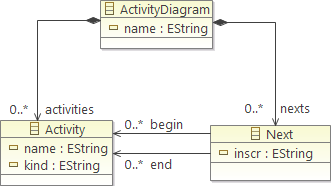
\includegraphics[scale=0.5]{./Figures/ActivityMetamodel.png}
    \rule{35em}{0.5pt}
  \caption[Metamodel of Activity Diagram]{Metamodel of Activity Diagram.}
  \label{fig:ActivityMetamodel}
\end{figure}

The metamodel of an activity diagram has an arbitrary number of activities and
next elements. An activity element can have a name and a kind. Example of
activity types can be decision or simple. The next element can have an
inscription and has the property to either start or end activities. The
collection of activities and next elements have to have an activity diagram
that they belong to. Now we have defined the metamodel that the source model
should conform to. To keep consistency between the models we need to have a
metamodel for the target model.

\begin{figure}[htbp]
  \centering
    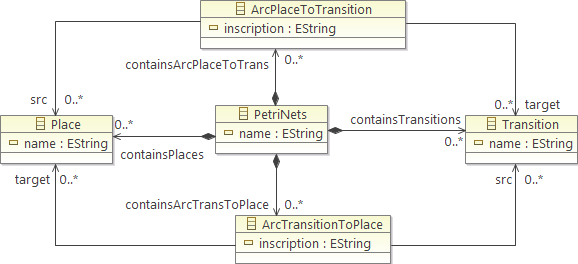
\includegraphics[scale=0.5]{./Figures/PetriNetsMetamodel.png}
    \rule{35em}{0.5pt}
  \caption[Metamodel of Petri nets.]{Metamodel of Petri nets.}
  \label{fig:ActivityMetamodel}
\end{figure}

The metamodel for a petri net consist of places and transitions. A petri net
instance must have a place connected to a transition or the other way around.
But a petri net can never have two of the same types connected with each other.
To solve this, the petri net metamodel has two nodes that specify if the
connection is between a place and a transition or a transition and a place.

These two metamodels can we use as source and target metamodel for
both Henhin and ATL. 